% Preamble
\documentclass[12pt]{article} % Sets the document class and font size

% Packages
\usepackage[utf8]{inputenc} % Input encoding
\usepackage[T1]{fontenc} % Output encoding
\usepackage{geometry} % Page layout
\usepackage{graphicx} % Include images
\usepackage{hyperref} % Interactive links and URLs
\usepackage{svg}


\geometry{
  a4paper, % Paper size
  margin=1in, % Margin size
}

\title{Mentora App Database Schema \& Report\\ Project Stage 01}

\author{Muhammad Rehan | 22P-9106}
\date{\today}

\begin{document}

\maketitle
\section*{Database Schema Overview}
The Mentora app's database schema is make to underpin an interactive educational app, having five essential entities: \textbf{Users}, \textbf{Posts}, \textbf{Comments}, \textbf{Courses}, and \textbf{Study\_Sessions}. The Study Sessions feature is optional right now. I am currently considering integrating it into the main functionality, but I might drop it later. This schema facilitates a techincally sound app, which is crucial for the app's educational objectives.

\begin{figure}[ht]
  \centering
  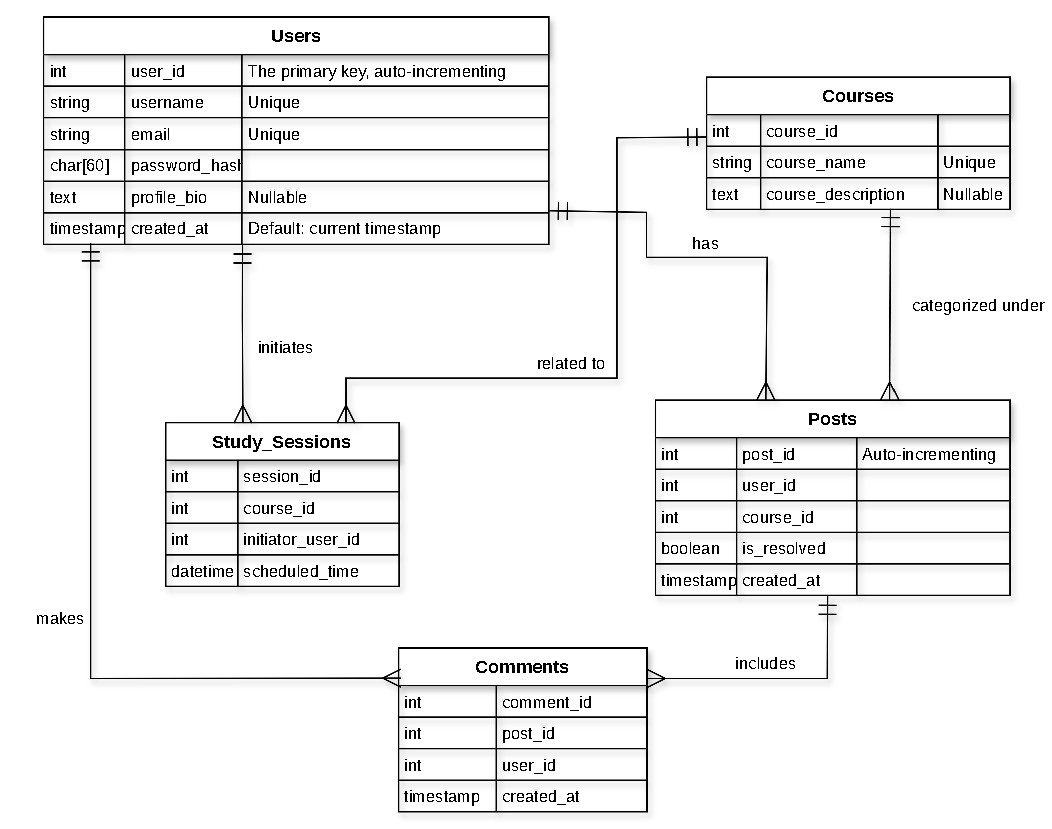
\includegraphics[width=\linewidth]{1.pdf}
  \caption{Database ERD Diagram}
  \label{fig:ust}
  \end{figure}

\section*{Detailed Entity Descriptions}

\subsection*{Users Table}
\begin{itemize}
    \item \texttt{user\_id}: Auto-incrementing primary key, ensuring unique identification.
    \item \texttt{username} and \texttt{email}: Enforced uniqueness supports authentication and user interaction.
    \item \texttt{password\_hash}: Secure storage of user credentials using bcrypt.
    \item \texttt{profile\_bio}: Optional bio, enhancing user profile customization.
    \item \texttt{created\_at}: Records the time of account creation, defaulting to the current timestamp.
\end{itemize}

\subsection*{Posts Table}
\begin{itemize}
    \item \texttt{post\_id}: Primary key, auto-incrementing for unique identification.
    \item \texttt{user\_id} and \texttt{course\_id}: Foreign keys that link posts to users and specific courses, fostering content organization and user interaction.
    \item \texttt{is\_resolved}: Facilitates the tracking and filtering of queries or discussions based on their resolution status.
    \item \texttt{created\_at}: Essential for organizing posts chronologically.
\end{itemize}

\subsection*{Comments Table}
\begin{itemize}
    \item \texttt{comment\_id}: Primary key for unique comment identification.
    \item \texttt{post\_id} and \texttt{user\_id}: Establish connections between comments, posts, and users, enriching the interactive experience.
    \item \texttt{created\_at}: Timestamp for tracking comment chronology.
\end{itemize}

\subsection*{Courses Table}
\begin{itemize}
    \item \texttt{course\_id}: Unique identifier for courses, serving as a primary key.
    \item \texttt{course\_name}: Unique naming facilitates course identification and organization.
    \item \texttt{course\_description}: Offers additional insights into the course content, optional for flexibility.
\end{itemize}

\subsection*{Study Sessions Table}
\begin{itemize}
    \item \texttt{session\_id}: Primary key for session identification.
    \item \texttt{course\_id} and \texttt{initiator\_user\_id}: Link sessions to specific courses and users, supporting structured study engagements.
    \item \texttt{scheduled\_time}: Specifies when study sessions occur, crucial for planning and attendance.
\end{itemize}

\textit{Please keep in mind that the database layout outlined here is preliminary and may undergo changes as the Mentora app development progress. As I develop the app further, adjustments to the database design may be needed to better accommodate user needs and new features. Think of this schema as a flexible foundation that I'll refine as I progress.}

% Document ends
\end{document}
